\chapter{Project Execution}
\label{chap:project_execution}

\section{Data Acquisition}
\label{sec:data_acquisition}

The project uses the full \textbf{UA-DETRAC} multi-vehicle tracking benchmark \cite{wen2020uadetrac}, consisting of $100$ real-world traffic video sequences recorded at $25\text{ fps}$ with resolution $960 \times 540$ pixels across urban road intersections, highways, and overpasses. Table~\ref{tab:dataset_stats} summarizes the exact statistics verified by \texttt{scripts/stats.py}.

\begin{table}[htbp]
    \centering
    \caption{UA-DETRAC dataset statistics and camera-location split (\texttt{data/stats.json})}
    \label{tab:dataset_stats}
    \begin{tabularx}{\textwidth}{l r X}
        \toprule
        \textbf{Property} & \textbf{Value} & \textbf{Verification / Notes} \\
        \midrule
        Total Video Sequences & $100$ & $60$ source-train + $40$ source-test sequences ($960\times 540$) \\
        Annotated Frames & $140,096$ & $89,109$ dense traffic frames containing $\ge 10$ simultaneous vehicles \\
        Total Vehicle Trajectories & $8,384$ & Track length percentiles: $P_{10} = 31$, $P_{50} = 91$, $P_{90} = 291$ frames \\
        Total Vehicle Bounding Boxes & $1,802,853$ & Classes: \textit{car, bus, van, others} \\
        Human / Pedestrian Boxes & $\mathbf{0}$ & Strictly non-human vehicle tracking verified across all $100$ sequences \\
        Train Split (Camera-Separated) & $48$ seqs & $44$ distinct camera viewpoint clusters ($120,000$ sampled training events) \\
        Validation Split (Camera-Separated) & $12$ seqs & $10$ distinct camera viewpoint clusters ($6,000$ fixed validation events) \\
        Test Split (Locked until Day 7) & $40$ seqs & $37$ distinct camera viewpoint clusters ($12,000$ locked test events) \\
        \bottomrule
    \end{tabularx}
\end{table}

To prevent background/viewpoint leakage between training and validation, \texttt{scripts/group\_locations.py} computes a $64 \times 36$ grayscale median background image for every sequence and applies Agglomerative Clustering ($\ell_1$ distance threshold $0.12$) so that sequences sharing the same camera viewpoint are never split across train and validation. Furthermore, for every bounding box, \texttt{scripts/extract\_hist.py} crops the inner $60\%$ region (reducing road background contamination) and extracts a 128-bin HSV histogram ($16\text{ H} \times 4\text{ S} \times 2\text{ V}$, $\ell_1$-normalized and cached as \texttt{uint8} in \texttt{data/cache/hist/\{seq\}.npy}).

\section{Training Methodology}
\label{sec:training_methodology}

\textbf{Mathematical Formulation of GapLink-Lite.} Given $N \le 6$ lost vehicle tracks and $M \le 10$ candidate detections at frame $t_{\text{conf}}$, GapLink-Lite computes a doubly stochastic assignment distribution over an augmented $(N+1) \times (M+1)$ matrix:
\begin{enumerate}
    \item \textbf{Scale-Normalized Kinematics \& Motion Encoder:} For each lost track $i$ with history length $L_i \in [1, 20]$ ending at $t_{\text{lost},i}$ and last bounding box $b_{i,L_i} = (c_x, c_y, w_l, h_l)$, each historical step $t$ is represented by 9 scale-invariant features normalized by $h_l$: relative displacements, velocities, accelerations, log-size ratios, aspect ratio, and normalized step index. A 2-layer GRU ($d = 128$) encodes the sequence into hidden state $h_i \in \mathbb{R}^{128}$, while the occlusion gap $g_i = t_{\text{conf}} - t_{\text{lost},i}$ is embedded via $\phi(g_i) = [\ln(1+g_i), g_i/90, \mathbb{I}(g_i\le 15), \mathbb{I}(16\le g_i\le 45), \mathbb{I}(g_i>45)] \in \mathbb{R}^5$ and projected to $g_{\text{emb},i} \in \mathbb{R}^{32}$.
    \item \textbf{Symmetric DeepSets Context Encoder:} Up to $N_{\text{ctx}} = 8$ surrounding vehicles within radius $5 h_l$ at $t_{\text{lost},i}$ ($\text{flag}=0$) and at $t_{\text{conf}}$ ($\text{flag}=1$) are encoded by a shared MLP followed by permutation-invariant max-plus-mean pooling into $c_i \in \mathbb{R}^{128}$.
    \item \textbf{Constant-Velocity Anchor + Residual Gaussian Predictor:} Using the constant-velocity anchor $\hat{\mu}^{\text{CV}}_i = v_i \cdot g_i / h_l$, the predictor outputs normalized residual mean and diagonal log-variance:
    \begin{equation}
        \mu_i = \hat{\mu}^{\text{CV}}_i + f_{\mu}(h_i, c_i, g_i), \qquad \ln \sigma_i^2 = \text{clamp}\big(f_{\sigma}(h_i, c_i, g_i), -6.0, 4.0\big)
    \end{equation}
    \item \textbf{Pairwise \& Competitive Dustbin Scorer:} For each track--candidate pair $(i, j)$ with normalized target offset $y_{ij}$, Gaussian log-density anchor $m_{ij} = -\frac{1}{2}\sum_{k=1}^4 \big(\ln \sigma_{i,k}^2 + (y_{ij,k} - \mu_{i,k})^2 / \sigma_{i,k}^2\big)$ is combined with center Mahalanobis distance, predicted box IoU, size-ratio differences, and HSV histogram cosine similarity into pairwise logit $S_{ij}$. Crucially, the track dustbin logit $z_i^t$ and candidate dustbin logit $z_j^c$ receive image-border proximity, appearance descriptors, and competitive summary statistics ($\max_j S_{ij}$, $\max_j \text{IoU}_{ij}$, $\max_j \cos_{ij}$) so the network can accurately abstain when a track exits the frame or remains occluded.
    \item \textbf{Log-Domain Sinkhorn Optimal Transport:} Forming the $(N+1)\times(M+1)$ score matrix $\tilde{S}$ with last column $z^t$, last row $(z^c)^\top$, and corner $0$, we run $T = 20$ alternating log-sum-exp row and column normalizations with target marginals $\mathbf{r} = [1, \dots, 1, M]^\top$ and $\mathbf{c} = [1, \dots, 1, N]^\top$ to obtain $\log P$.
\end{enumerate}

\textbf{Joint Loss Function \& Curriculum Training.} The model is trained with AdamW ($\text{lr} = 5\times 10^{-4}$, cosine annealing after 300 warmup steps, batch size $64$, $6,000$ steps, gradient clipping $1.0$) on an NVIDIA GeForce RTX 3050 6GB Laptop GPU using the joint objective:
\begin{equation}
    \mathcal{L} = w_{\text{assign}} \mathcal{L}_{\text{assign}}(\log P, y^t, y^c) + w_{\text{nll}} \mathcal{L}_{\text{NLL}}(\mu, \ln \sigma^2, y^*)
\end{equation}
where $w_{\text{assign}} = 1.0$, $w_{\text{nll}} = 0.5$, and curriculum sampling increases the fraction of geometrically hard events from $40\%$ to $80\%$ over the first $60\%$ of training. Total training time for the 6,000-step main run was $250.2\text{ seconds}$ ($4.2\text{ minutes}$).

\section{Workflow}
\label{sec:workflow}

To guarantee zero train--test skew between event-level training and online multi-object tracking, both the training sampler and Stage-2 of the online tracker call the exact same pure function \texttt{assemble\_event} (verified to bit-level numerical identity by \texttt{tests/test\_parity.py}). During online tracking on a sequence:
\begin{itemize}
    \item \textbf{Stage 1 (Active Track IoU Association):} Active tracks ($\text{age} = 0$) are matched to current-frame detections using pairwise bounding-box IoU and the Hungarian algorithm with threshold $\text{IoU} \ge 0.30$.
    \item \textbf{Stage 2 (Occlusion Gap Re-Association):} Unmatched detections and lost tracks with $2 \le \text{age} \le a_{\max}$ ($a_{\max} = 60$) are assembled into an event tensor and passed to the associator (C-2, C-3, C-4, or GapLink-Lite). For GapLink-Lite, Hungarian matching is applied to $-P_{1:N, 1:M}$ and a link $(i, j)$ is accepted if and only if $P_{ij} \ge \tau$ ($\tau = 0.20$ selected on validation) and $P_{ij} > P_{i, M+1}$ (real candidate probability strictly exceeds dustbin probability).
\end{itemize}

\section{System Design}
\label{sec:system_design}

Figure~\ref{fig:system_design} illustrates the end-to-end architecture of GapLink-Lite and its integration within the two-stage online vehicle tracker.

\begin{figure}[htbp]
    \centering
    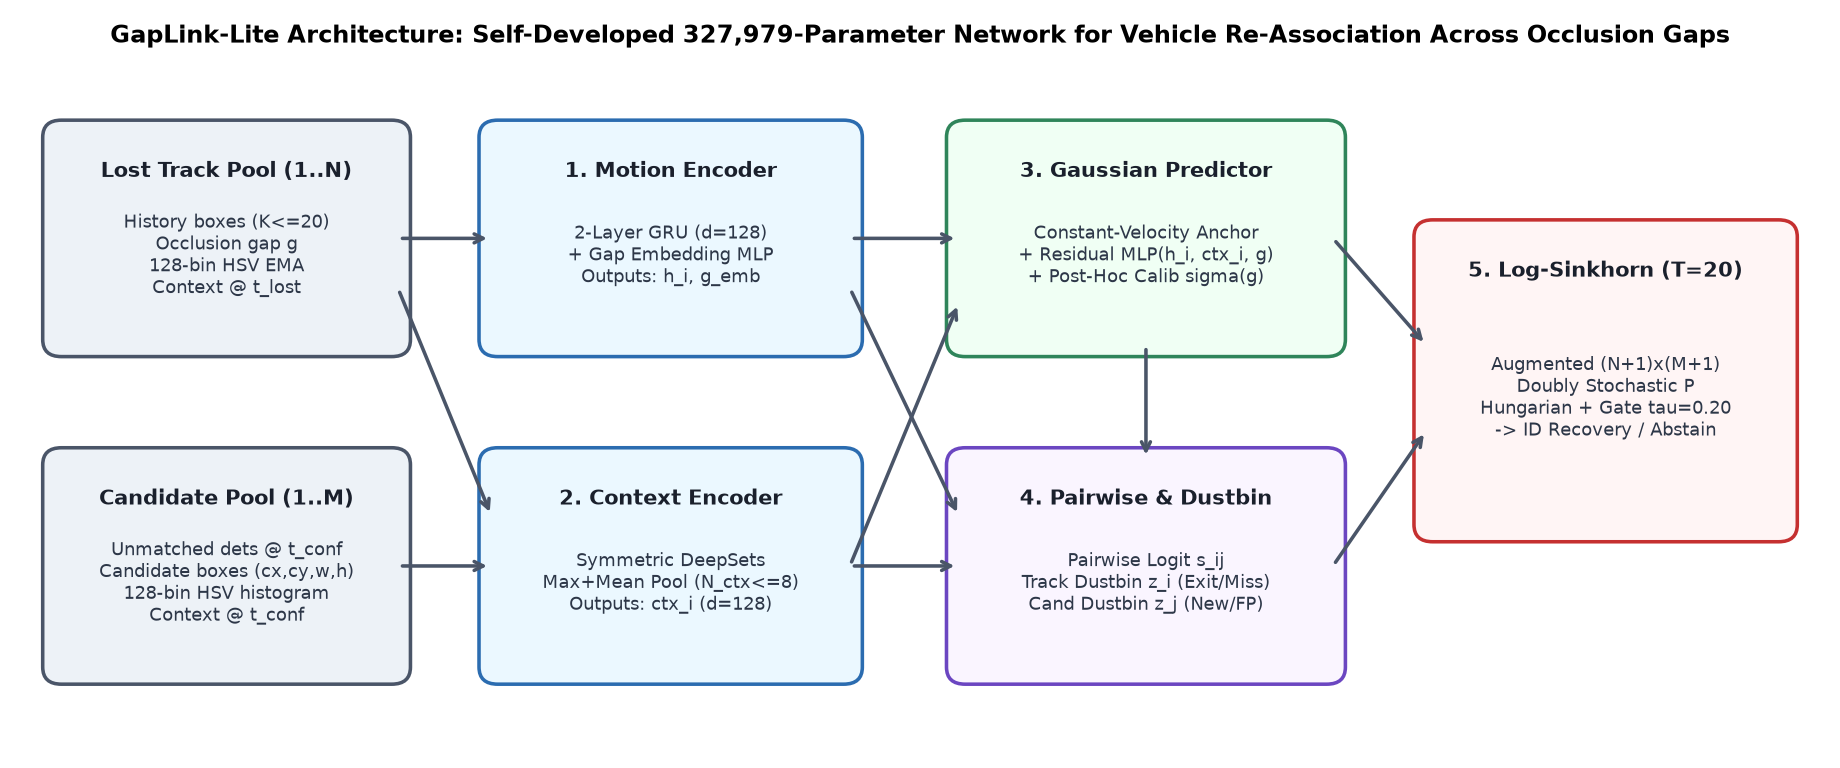
\includegraphics[width=0.98\textwidth]{figures/fig_system_architecture.png}
    \caption{Overall System Architecture of GapLink-Lite ($327,979$ parameters) and 2-Stage Online Vehicle Tracker}
    \label{fig:system_design}
\end{figure}
